\chapter{Adult-Led OurPlace Engagements}
\label{chap:Teachers}

\section{Overview}

As well as investigating how mobile learning platforms such as OurPlace could be used by community experts and stakeholders for sharing their knowledge and values, we were also interested in exploring if and how such tools could work within a formal education context. To this end, at the same time as working with the community heritage groups we were also working with teachers to investigate the use of ParkLearn as a seamless, place-based learning tool, garnering feedback as to how the application could be improved. This involved a longitudinal study with a local primary school, as well as several one-off studies with other schools in the area. The longitudinal study was a part of a body of work which was peer-reviewed and published at MobileHCI 2018 \citep{Richardson2018}, with the paper being co-authored by Doctors Pradthana Jarusriboonchai, Kyle Montague and Ahmed Kharrufa. Sections \ref{sec:SenseExplorers} and \ref{sec:TyneFresh} describe studies held by Sean Peacock and Sebastian Prost, respectively, in which OurPlace was used with schools during other research projects.

As some of these studies were running concurrently with the community engagements covered in Chapter \ref{chap:Community}, the application still existed as `ParkLearn' for a large number of them, without the features and re-branding of `OurPlace'. This Chapter will describe the engaged school as a research context; how we introduced ParkLearn to the teachers; how the teachers introduced the app to the students; the Activities that the teachers created; observations and discussion of the application's use in this context; and a brief overview other schools' usage of the app in other studies.

\section{Longitudinal Study Context}
\label{sec:LongitudinalSchool}

I was put into contact with a teacher at a local primary school through a co-researcher, Dr Jarusriboonchai, who was working with them on a different research project. Aiming to to evaluate and further develop the ParkLearn application according to the design goals (DGs) covered in Section \ref{sec:DesignGoals}, I worked with this teacher (Teacher 1, Year 4---aged 6-7) for a period of roughly one year, using ParkLearn multiple times on school trips, in the classroom and on the school's grounds. I also worked with another teacher (Teacher 2, Year 6---aged 10-11) in the same school, although this was limited due to examination pressures. 

The longer study period was chosen for two main reasons: to mitigate the influence of `novelty' in the children’s engagement with the technology (the hope was that once students had used the application multiple times, more authentic engagement could be observed---rather than simply excitement at the chance to use new technology) \citep{Sharples2013} and to see how the teachers' approaches to Activity creation would change as they gained experience with the application over time. To this end, rather than have the research team create Activities for the students complete, the teachers used the application at their own volition: they took on a co-researcher role, creating the ParkLearn Activities independently and developing their own design ideas. The teachers chose to use the application a total of eleven times between the two classes during the study period: twice with the Year 6 class, and nine times with Year 2.

The school is situated in one of the most economically deprived areas of England: the ward in which the school sits features the highest crime rate within the constituency, 26\% of its population are within the 10\% most deprived in the UK, and 15\% of the children within the ward live in poverty (down from 27\% in 2010). The area's life expectancy is 73 years for people born male, and 78 for people born female---significantly lower than the national average of around 88 years.

Teacher 1 claimed that the school had particular difficulty in engaging with many of the students' parents, many of whom were unlikely to appear at parents' evenings or other similar school events (for example, only two parents attended a meeting about a class's transition between school Key Stages). Despite this, the school itself is of a very high standard, having been awarded an `Outstanding' rating in their latest Ofsted (the UK’s Office for Standards in Education) review. While they don't have access to their own transportation (having to instead hire coaches), the school lies within a short driving distance of the park referred to in Section \ref{sec:TalkingStatue}. It also features its own grounds, including a tarmacked playground, sizable green space and a small wooded area.

As this was a primary school, teachers each teach individual classes for all subjects, including technology-related subjects. While Teacher 1 was not very confident in using digital technology, Teacher 2 was seen as the school's `whizz-kid' teacher. As they taught a slightly older class of students, Teacher 2 frequently tasked them with doing online research during classroom activities. To this end, the school had within recent years established a partnership with Samsung, who had supplied them with a smart classroom display and 20 Android tablets, which were a shared resource amongst all the school’s classes. While a shared resource, the older classes were given priority, and Teacher 2's class regularly used them during classroom activities. However, as there were typically fewer tablets than there were children per class (typically ~30), tablets were often shared between pairs of students.

\section{Introducing the Application}

Prior to the application being used in class, we sat down with the teachers for an hour to give them a brief overview of the study, the application itself and how we had imagined it could be used. To serve as examples for what the app could be used for, we had created two simple Activities beforehand. The first Activity took the learner on a bug hunt, using primarily camera-related Task Types to find and photograph insects in an outdoor environment. The second Activity was a more creative one about movie making, and involved the learner creating materials for their own film (such as recording `Foley' sound effects, designing a poster and recording videos of specific shots). While Teacher 2 understood the ParkLearn application very quickly and didn't feel the need to engage with it very much, Teacher 1 took longer to be comfortable with it due to their lack of confidence around digital technology. However, it wasn't long before Teacher 1 also understood the app, and they were enthusiastic about using it independently: after going through the example materials, they created their own short Activity containing a \textit{Location Hunt} and several \textit{Match Photos}, going outside onto the school grounds to take the target photos and try out the created Activity. 

We let the teachers decide how they would like to introduce the students to the app, and they decided to create a simple Activity together for use in introductory lessons with their respective classes. Their first Activity was very exploratory, designed for use in the classrooms to see how easily the children could use the application (Table \ref{tab:TeacherActivities}, row 2). This Activity focused mainly on camera-related Task Types, as the teachers perceived them to be more immediately understandable interactions and could be easily completed in the classroom environment. In contrast, while they were excited by \textit{Location Hunt}, the teachers were worried that the distance measurement would be too abstract for some of the children (particularly the younger ones), and it would require the introductory session to be held outside. This session was as much for the teachers to get used to using the application as it was for the students---the teachers were able to practice instructing the students on how to open a particular Activity (opting to use the share code, rather than display a QR code), and see how the students' responses could be uploaded and viewed after the session.

The introductory sessions with the two classes went well, and by the end of them the children largely understood the ParkLearn app. For the Year 6 children, this may have been because they were already extremely comfortable with using the tablets and familiar with standard Android application interfaces, and so had very few issues understanding the application’s design language. However, some of the younger Year 4 children were less able readers, and so struggled to understand even the simple instructions for each Task created by the teacher. To mitigate this, subsequent versions of the ParkLearn app featured the text-to-speech function, which read aloud the Task’s instruction at the push of a button available on each Task's card.

\begin{table}[]
    \centering
    \begin{tabularx}{\linewidth}{ 
| p{4mm} 
| >{\raggedright\arraybackslash}X 
| >{\raggedright\arraybackslash}X 
| p{13mm}
| >{\raggedright\arraybackslash}X 
| >{\raggedright\arraybackslash}X 
|}
\hline
\small\textit{\#}
    & \small\textit{Activity Title} 
    & \small\textit{Used Task Types}
    & \small\textit{Uploads}
    & \small\textit{Uploads' Cumulative Contents}
    & \small\textit{Notes}\\
\hline
\small 1 
    & \footnotesize `Our School Grounds' 
    & \footnotesize 2 Record Audio; 1 Take Photos; 1 Record Video; 1 Photo Match 
    & \footnotesize 1  
    & \footnotesize 2 audio recordings; 2 photos; 1 video
    & \footnotesize Only used by Teacher 1 to test the application\\
\hline
\small 2
    & \footnotesize `Learning to use ParkLearn' 
    & \footnotesize 3 Take Photos; 1 Draw on Photo; 1 Record Audio; 1 Record Video 
    & \footnotesize 29  
    & \footnotesize 91 photos; 29 drawings; 29 audio recordings; 29 videos
    & \footnotesize Used in the classroom by both teachers to introduce the children to ParkLearn\\
\hline
\small 3
    & \footnotesize `Trip to X Hall and Gardens' 
    & \footnotesize 2 Take Photos; 2 Photo Match; 1 Record Audio; 1 Record Video; 1 Map Marking; 1 Location Hunt 
    & \footnotesize 8  
    & \footnotesize 43 Photos; 8 audio recordings; 8 videos
    & \footnotesize Tablets shared in pairs\\
\hline
\small 4 
    & \footnotesize `X Park---Statues and Monuments' 
    & \footnotesize 4 Take Photos; 2 Record Audio; 1 Record Video
    & \footnotesize 0  
    & \footnotesize -
    & \footnotesize Responses weren't uploaded\\
\hline
    \small 5 
    & \footnotesize `Exploring X Park's Flower Garden' 
    & \footnotesize 5 Photo Match; 2 Take Photos; 1 Record Video
    & \footnotesize 5 
    & \footnotesize 46 photos; 5 videos
    & \footnotesize Some submissions were lost as tablets were re-used prior to upload\\
\hline
    \small 6 
    & \footnotesize `X Park---First Visit' 
    & \footnotesize 9 Photo Match; 1 Take Photos; 1 Record Video; 1 Record Audio
    & \footnotesize 7 
    & \footnotesize 78 photos; 7 videos; 7 audio recordings
    & \footnotesize Some submissions were lost due to software bug\\
\hline
    \small 7 
    & \footnotesize `KS1 Tree Day' 
    & \footnotesize 5 Photo Match; 1 Record Audio; 1 Text Entry; 1 Take Photos
    & \footnotesize 15 
    & \footnotesize 67 photos; 15 audio recordings
    & \footnotesize Children asked to enter their names in the Text Entry Task\\
\hline
    \small 8 
    & \footnotesize `Zoological Gardens' 
    & \footnotesize 6 Take Photos; 1 Record Video; 1 Record Audio
    & \footnotesize 12 
    & \footnotesize 173 photos; 12 videos; 12 audio recordings
    & \footnotesize n/a\\
\hline
    \small 9 
    & \footnotesize `Welcome to Class 2' 
    & \footnotesize 2 Record Video; 1 Take Photos; 1 Record Audio
    & \footnotesize 4 
    & \footnotesize 8 videos; 7 photos; 4 audio recordings
    & \footnotesize n/a\\
\hline
    \small 10 
    & \footnotesize `Year 2 at X Keep' 
    & \footnotesize 1 Record Video; 1 Take Photos;
    & \footnotesize 5 
    & \footnotesize 5 videos; 13 photos;
    & \footnotesize One of the responses was from the site's manager\\
    \hline
    \small 11 
    & \footnotesize `X Zoo 2018' 
    & \footnotesize 1 Record Video; 1 Take Photos;
    & \footnotesize 13 
    & \footnotesize 10 videos; 98 photos;
    & \footnotesize n/a\\
\hline
\end{tabularx}
    \caption[The Activities created by teachers 1 and 2, and the uploaded responses created by students.]{The Activities created by teachers 1 and 2, and the uploaded responses created by students. Rows 1 and 4-11 were created by Teacher 1, row 3 by Teacher 2, and row 2 by both.}~\label{tab:TeacherActivities}
\end{table}

\section{Year 6 Activities}

The Year 6 (aged 10-11, we engaged N=16 children) group used the application on a trip to a site popular with school groups thanks to its historical, natural and scientific features. The site featured an indoor museum and a large outdoor property featuring woodlands and ornamental gardens. As the location was a significant distance away from the school, the teacher was unable to visit the site to create the Activity in-situ. Instead, Teacher 2 prepared the Activity (Table \ref{tab:TeacherActivities}, row 3) independently on their own device the night before, designing it using online resources in combination with their prior knowledge of the location. For Task Types which required additional resources, the teacher downloaded them from the Internet rather than collecting them personally (e.g. using photographs downloaded from Google Images for \textit{Photo Match} Tasks). Using the Activity's share code, the teacher asked the students to pre-load it in the classroom while an Internet connection was still available, prior to the class leaving. Students shared the tablets one between two, with 8 tablets being used (the class was split into two groups of 15-16, with only one group using the app). 

The Activity's Tasks included: \textit{Take Photos} of the various wooden bridges present; \textit{Photo Match} Tasks of a modern water pump and an iron bridge; a \textit{Record Audio} of the natural sounds of the forest; a \textit{Record Video} of an Archimedes screw rotating; a \textit{Map Marking} Task to plot where the site's powerhouse was; a \textit{Location Hunt} to navigate the children to a mystery location (an old waterwheel); and a final Task which challenged the children to compete and \textit{Take Photos} of the most beautiful flower they could find. Unfortunately, the teacher's \textit{Map Marking} Task didn't work during the trip, due to the Task Type's reliance on Internet connectivity to load Google Maps.

Unfortunately, due to the class entering into an examination period, this was the only time that Teacher 2 was available to use ParkLearn during the study.

\section{Year 2 Activities}

After the introduction session, the Year 2 class (aged 6-7, N=29) used ParkLearn on three separate school trips, as well as during multiple activities on the school grounds. For the class's first trip to the park, Teacher 1 created two different Activities at home, independently on their own device. The first focused on the historical monuments and memorials in the park, and asked the children to record videos of each other explaining what each monument was dedicated to (Table \ref{tab:TeacherActivities}, row 4). The second Activity used \textit{Photo Match} Tasks to find and photograph specific flowers in the park, with a final \textit{Take a Photo} Task asking them to choose their favourite (Table \ref{tab:TeacherActivities}, row 5). These Activities largely focused on camera-based interactions, as Teacher 1 believed that the younger Year 2 children would be able to more easily understand them than the more complicated Task Types. The students didn't find the first Activity very engaging, and the teacher and assistants resorted to telling the children what to say when recording the videos. Unfortunately, many of the children's responses to these Activities were lost: Teacher 1 didn't see much value in the responses to the first Activity, and so didn't upload them. The students engaged more with the second Activity, however much of the data was wiped by students re-using tablets (this early version of the app didn't wipe Activities after finishing, ready for re-use---that feature was added in response to this).   

Teacher 1 also used the application on another trip to different local park, where the park ranger had invited their class to make suggestions as to how the it should be improved. Independent of the research team (we only found out after the trip had taken place), the teacher made another Activity which asked the students to take photos of different areas of the park, and make audio recordings which would then be shared with the park ranger (Table \ref{tab:TeacherActivities}, row 6). Unfortunately, a bug in this version of the app resulted in a loss of several children’s work, meaning that these children’s feedback was sent to the ranger as part of a classroom writing exercise instead. Teacher 1 resorted to sharing their Google account details in order to share the children's uploads with the ranger. In response, I added the ability to share `magic links' to uploaded responses on the website, which didn't require the recipient to log into the platform (as described in Section \ref{sec:ImplementationWeb}).

The Year 2 class also used the application during the school's `Key Stage 1 Tree Day', using it to identify and talk about the trees they could find on the school's ground. Teacher 1 created an Activity which included a variety of Tasks, from \textit{Photo Match} Tasks which asked students to find particular tree types, to a \textit{Record Audio} which asked the children to describe how it felt to be around nature (Table \ref{tab:TeacherActivities}, row 7). By this point Teacher 1 was getting familiar with how the app worked, and had realised that because all of the students' devices were logged into the same account, identifying who uploaded what could be difficult. As a solution, the teacher included a \textit{Text Entry} Task into this Activity, and made sure that the children entered their names into it before starting the Activity. Following this, I added the ability for Activity creators to require a name entry field be completed prior to respondents uploading results, the contents of which would be visible on the `Your Uploads' and `Responses' pages on the website (as described in Section \ref{sec:ImplementationWeb}).

\begin{figure*}
  \centering
  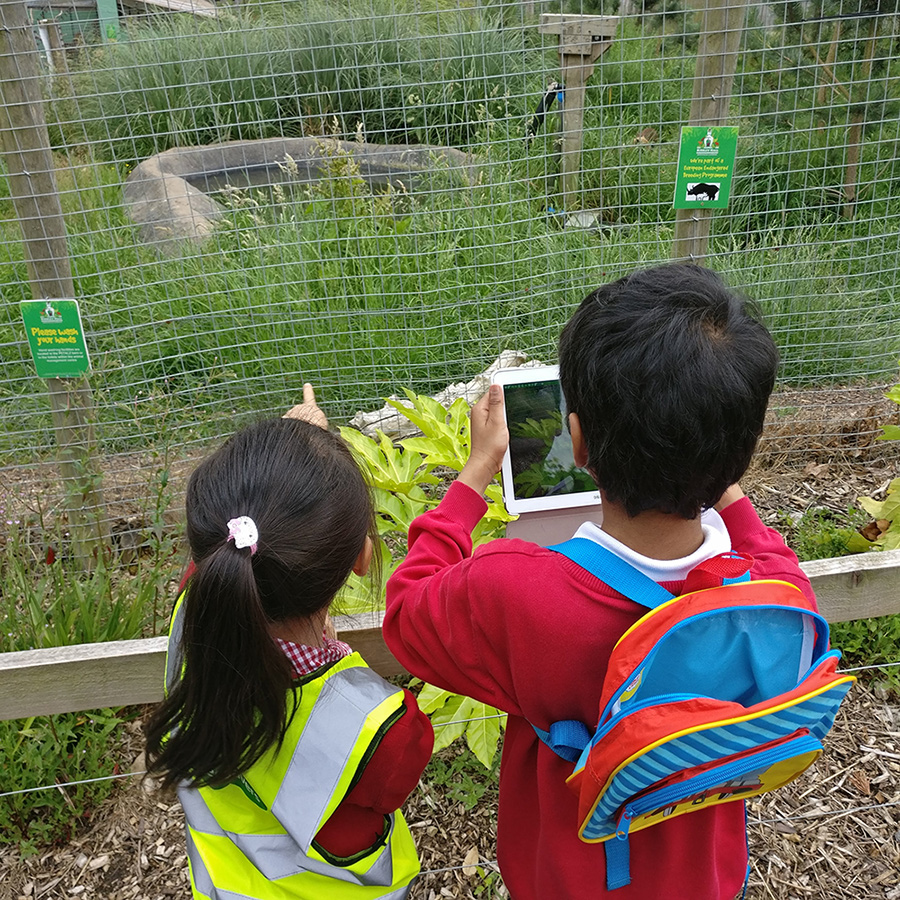
\includegraphics[width=0.7\columnwidth]{images/chapter07/zoo.jpg}
  \caption[Children using ParkLearn during a class trip to the zoo]{Children using ParkLearn to classify zoo animals during a class trip (using Teacher 1's Activity detailed in Table \ref{tab:TeacherActivities}, row 8)}~\label{fig:ParkLearnZoo}
\end{figure*}

The teacher also used the application on a class trip to the zoo (Figure \ref{fig:ParkLearnZoo}), with a simple Activity consisting of Tasks which asked the children to take photos of animals, categorizing them into different types. The Activity then asked the students to record video clips, asking them to present a fact of their choice that they had discovered during the day and found particularly interesting (Table \ref{tab:TeacherActivities}, row 8).

The class' final use of the app took place at the end of the school year. Teacher 1 created an Activity which asked four children from the class to give advice to the younger Year 1 students about being in Year 2 (Table \ref{tab:TeacherActivities}, row 9). The Activity asked the children to choose and photograph an area of the classroom, and record a video giving advice about the do’s and don’ts. The teacher chose these four children either because they would benefit from the practice (due to a lack of confidence or, in the case of ‘Child 1’, a speech impediment), or because they were especially enthusiastic about using ParkLearn again. Once the children's responses were uploaded, the teacher played their videos to the class on the classroom's projector via the ParkLearn website.

Teacher 1 went on to use the application twice with the new Year 2 class the following academic year, by which time the app had been re-branded to OurPlace. The first time this new class used the app was during a trip to a medieval castle, for which the teacher had prepared a very simple Activity consisting of only two Tasks: a \textit{Take Photos} and a \textit{Record Video} (Table \ref{tab:TeacherActivities}, row 10). Due to the space limitations of the castle's cramped rooms, the class was split into two groups---one of which were given tablets with OurPlace loaded onto them. Unfortunately, the tablets weren't used much, due to the students having hands-on activities and tours with the castle staff (Teacher 1 didn't want the students to disrupt the tour through being distracted by the tablets). As a result, not many responses were uploaded by the students. Over a year later, however, one of the castle staff found the Activity (it had been tagged as being at the castle, and so was discoverable by location) and recorded his own responses to Teacher 1's two Tasks.

The final Activity created by Teacher 1 was for the new class's trip to the same zoo as the previous year . While the previous Activity for that location was somewhat structured (with multiple goals for \textit{Take Photos} Tasks), the teacher instead decided to make the new Activity as open as possible, simply asking the students to take photos and videos of things which interested them (Table \ref{tab:TeacherActivities}, row 11). Again, the class was split into two groups, with only one half having access the the OurPlace app. The number of photos uploaded averaged around 8 per student, less than the previous year's Activity, which averaged around 14 photos.

\section{Findings \& Observations of the Teachers' Use of ParkLearn \& OurPlace}

For the ease of presentation, the observation and interview data from this longitudinal study has been structured into the three themes that emerged from the thematic analysis of the engagements held with the school: \textit{Supporting Seamless Learning Practices}; \textit{Engagement and Empowerment Through Ownership}; and \textit{Supporting Civic Engagement and Inquiry}. This section will cover the observations and data relating to these themes, for discussion in Section \ref{sec:TeacherDiscussion}.

\begin{figure}
    \centering
    \begin{tikzpicture}
    \pie[explode=0.2, text=pin, radius=3.5]{
    12/Record Audio,
    34/Take Photos,
    2/Draw on Photo,
    16/Record Video,
    34/Photo Match,
    2/Text Entry}
    \end{tikzpicture}
    \caption[Teacher 1's usage of Task Types across their created Activities]{Teacher 1's usage of Task Types across their created Activities, including the Activity made alongside Teacher 2.}
    \label{fig:TaskTypeUsage}
\end{figure}

\subsection{Supporting Seamless Learning Practices}

Children in both age groups were easily able to use the application to independently collect data, allowing them to make the most of being in the field. The application's ability to support children responding through multimedia (images, video, audio) allowed for them to immediately collect data and record their reflections on it, without struggling with poor writing skills and virtual keyboards. This was especially true with the younger children, many of whom weren't strong writers (especially when tasked with writing on virtual keyboards). When (during a semi-structured interview midway through the study) Teacher 1 was asked about why they chose certain Task Types, they revealed that they had purposefully chosen ones which wouldn't be technically challenging, allowing children to focus on the Tasks' content rather than struggling with interacting with the technology itself: 

\begin{displayquote}
"It’s automatic. They can just speak. [...] When I designed the [‘\textit{Zoological Gardens}’] activity, I basically did the video, because I wanted them not to have to write."
\end{displayquote}

Teacher 1 particularly favoured use of the camera, taking up 84\% of their created Tasks (Figure \ref{fig:TaskTypeUsage}). The first class's interactions with the technology became more purposeful as the study progressed, unhindered by a lack of familiarity and the earlier versions' bugs. This was shown in the first trip to the zoo: the children were careful to correctly classify each animal into the correct Task, trying to take as good a photograph as possible and deliberately deleting and re-taking any shots that didn't meet their increasingly high standards. One pair of children even decided to re-shoot their video recording twice, in order to ensure their delivery of information was perfect. Despite this perfectionism, each pair still uploaded over 14 photos on average in addition to their audio and video recordings (Table \ref{tab:TeacherActivities}, row 8). Unfortunately the second Year 2 class didn't have anywhere as much time with the application, with only half of the class having access to the tablets for a whole trip, making it hard to compare. However, the older children also responded well to their Activity, particularly enjoying competing to take the best flower photo, the \textit{Location Hunt} Task’s sound and animation and competing to take the most accurate \textit{Photo Match}.

The `Welcome to Class 2' Activity proved to be a very different use-case for the application: in contrast to the other uses of the application---in which it tended to be used as the sole medium for the students' work---most of the learning process took place independent of the technology, as the children created their presentations and practiced with each other using whiteboards and markers. Rather than encompass the entirety of the activity workflow, in this case ParkLearn was used to bookend it: delivering instructions and prompts at the beginning to children for talking points, and at the end of the activity to record their final output for later viewing by the class and evidencing by the teacher. The ability to prepare and redo a video presentation without it being `live' and in front of an audience proved very effective for children such as Child 1, who Teacher 1 claimed would have normally struggled due to a lack of confidence. Reflecting on the activity after the session, the teacher stated that not only did the children enjoy recording the videos, but that they also took pride in sharing the final results: 

\begin{displayquote}
"[Child 1 would present his work], but he doesn't know what he’s going to say, he gets tongue-tied. The pride he’ll take in actually being able to give a coherent message and seeing himself back... They far more enjoyed what they were saying and what they were doing."
\end{displayquote}

While two of the children didn’t want to play back their videos for themselves immediately after recording them, all four participating children were eager to show their videos to the rest of the class afterwards. The other children reacted with excitement at seeing their classmates on the screen, with Child 1 even receiving high-fives.

The teachers saw great value in how simple the app made creating a structured learning activity, and then  collecting (and sharing) the children’s responses to it. When interviewed towards the end of the study, Teacher 1 noted that they found that the platform offered an approachable user experience which supported them in producing their own mobile learning activities, despite their lack of confidence with digital technology:

\begin{displayquote}
"It’s powerful, really powerful. The way that packages it up at the end, and how immediate it is, is fantastic for me. I got it straight away, it wasn't a difficult process to do."
\end{displayquote}

Prior to the study, the school’s teachers had been manually transferring the children’s created photos and videos over USB on a weekly basis, uploading the children’s media to `Earwig'---an evidence of learning portfolio suite used by the school. Teacher 1 argued that ParkLearn’s smaller output file sizes and upload pipeline was far simpler and better suited to their workflow:

\begin{displayquote}
"That simplicity takes away a lot of hassle---if I was to take photographs on my [tablet], I've got to get the lead, plug it into my hard drive, transfer the photos across, choose where I want to save them... Whereas this packages everything together."
\end{displayquote}

This one-step system took a fraction of the time compared to the old backup routine, meaning children’s creations would be discarded less often. Its simplicity even allowed the teachers to delegate uploading to the children. Teacher 1 also valued that the submissions appeared on the website in the same format as they appeared on the learner’s device: 

\begin{displayquote}
"What I like about the app is you can pull together different ways of collecting and showing information. Simply by pressing that upload button, it puts it onto my screen to save and to use in that format. That’s the beauty of it."
\end{displayquote}

Teacher 1 claimed that it was because the application's support for both open-ended and structured learning activities and non-intrusive workflow that they continued to use the application with the next class of students. When asked which school trips would benefit from this data collection, they responded: "\textit{Every trip.}" This was demonstrated by Teacher 1 then proceeding to use the app on two further occasions with the following cohort.

\subsection{Engagement and Empowerment Through Ownership}

Both teachers created Activities which ranged between being highly prescribed (e.g. A \textit{Photo Match} Task, asking students to ‘Find a birch tree’) and open-ended (e.g. A \textit{Take Photos} Task with ‘Find what you think is the most beautiful flower’). The Year 2 class's first Activity proved to be very prescriptive, with the teacher resorting to simply having the children repeat her words on video. While the children enjoyed recording each other with the tablets, they weren't very engaged with the actual educational content (suggesting a high influence of the technology’s novelty factor). The children's lack of enthusiasm was evident in the resulting videos, leading Teacher 1 to not bothering to uploading them. Furthermore, this prescriptive nature resulted in the children having less interest in viewing and sharing each others' outputs. Teacher 1 noted in an interview after the first zoo trip that in the cases where Activities leave the students with little creative control, the children were only really interested in viewing their own work: 

\begin{displayquote}
"When they come back after visits where we've all done the same, children's enthusiasm is not really there for what others have done. The enthusiasm is, `Can I see what I've done?'"
\end{displayquote}

When they \textit{were} engaged in the Activities and given some more creative control, the children took pride in the photos they had taken, and particularly enjoyed showing off their creations to each other and the adults present (both in-situ, as the Activity was being completed, and back in the classroom, when results were visible). In response to finding that the students were interested in viewing each others' work if it was independently and creatively produced, Teacher 1 started planning future activities which would involve the children having their own topics in small groups: 

\begin{displayquote}
"They’re given a specific task and they take ownership of it, knowing that other groups are not doing that. […] When we come back to school and we feedback, there’s a great interest in what each other has produced because we’re informing everybody."
\end{displayquote}

The teacher argued that having the students research and respond to their own topics would lead to the children becoming experts on it amongst their friends, allowing for peer-learning activities. They argued that having the students take ownership of the task and knowledge would be an empowering factor for them, boosted by the ability to teach their peers new knowledge:

\begin{displayquote}
"You can kind of empower yourself through your knowledge and how you’re going to present it, and then go off and do it."
\end{displayquote}


\subsection{Supporting Civic Engagement and Inquiry}

As well as for purely education tasks, Teacher 1 used the ParkLearn platform as a tool to facilitate civic participation during the class trip to the second park (Table \ref{tab:TeacherActivities}, row 6), with students providing feedback and suggestions to the park's ranger through the application. Engagement with the local community (including the children's families) through class activities was something that the school was keen to promote. Unfortunately, community engagement wasn't coming easily, with even the children's families not actively participating. Teacher 1 noted that the school was trying to engage with various cultures that could be found within the local community as learning resources, but had been struggling to get parents on board: 

\begin{displayquote}
"We don’t have a lot of parental support, but, where we do, we’re looking to make cultural links."
\end{displayquote}

After this trip to the park, she had tried to make the parents aware of their children’s active citizenship through the school newsletter. The teachers noted that their currently used technology, `Earwig', was impractical for this due to workflow issues such as slow upload speeds and manual data input. During an interview after this park trip, Teacher 1 claimed that as a result of these limitations the amount of digital content shared with parents by the teaching staff had dramatically reduced:

\begin{displayquote}
"It takes a very long time to upload a video within Earwig, so we've stopped doing it, really."
\end{displayquote}

However, Teacher 1 suggested that mobile nature of learning technologies such as ParkLearn may be better suited to highlighting the children’s civic engagements, as communities are able to access them in-situ, lending the children's work greater context: 

\begin{displayquote}
"Our parents might go along and just say, `There's nothing there', because they don’t see the resource. However, there could be something on the app like, `We're involved in it, so go along and see what your children have done.'" 
\end{displayquote}

Teacher 1 was particularly enthusiastic about the idea of using mobile learning technologies for civic learning, and sharing evidence of the children's civic engagements with the wider community. For example, they suggested using ParkLearn to highlight class visits to local care homes, recording the children's engagements and the elders' knowledge: 

\begin{displayquote}
"Let’s say, Christmas you go to the care home. We can use ParkLearn to record what we did and use that within school, upload it to our website to share it with parents."
\end{displayquote}

Taking this idea further, Teacher 1 extended it to conceptualise ParkLearn as a tool to facilitate cross-cultural learning engagements, with the technology acting as a medium for digital, place-based `pen-pals': 

\begin{displayquote}
"We have a link with a school in India. The app is a perfect way of interacting with them, showing each other."
\end{displayquote}

Beyond the civic engagement with the park ranger, Teacher 1 also used the ParkLearn platform as a medium to encourage the students in reflecting upon their experiences in place, and their relationship with space. For example, one Task in the `KS1 Tree Day' Activity asked children to record audio in response to the prompt:

\begin{displayquote}
`Why are trees special? Listen to the sound of the leaves rustling, stand amongst them and look up – how does it make you feel? Share your thoughts with us.' 
\end{displayquote}

While a large number of the children's responses gave an appreciation about many of the reasons trees were useful (e.g. food, fuel), some of them also included more personal reflections and metaphorical observations. For example, several children talked about how they "loved" the trees, and how it looked like they "dance" when there's a slight breeze.

\section{Longitudinal Study Discussion}
\label{sec:TeacherDiscussion}
These engagements provided several discussion points around how ParkLearn addressed the design goals set out in Section \ref{sec:DesignGoals}, as well as several other points which I believe should bear consideration in future designs for seamless mobile learning technologies. This discussion has been separated by the three themes produced through inductive thematic analysis, respective to the relevant data in the previous section. These themes are: \textit{Supporting Seamless Learning Practices}; \textit{Engagement and Empowerment Through Ownership}; and \textit{Supporting Civic Engagement and Inquiry}.

\subsection{Supporting Seamless Learning Practices}

The features and open nature of the application's authorship process and website component means that it arguably supports all ten of Wong and Looi’s dimensions of mobile-assisted seamless learning \citep{Wong2011}.  This includes the four research and design gaps which they identified: use of multiple device types in different contexts (demonstrated with ParkLearn, through use of tablets in the outdoors and the desktop and projector in the classroom), switching between multiple learning tasks (demonstrated by combining Task Types, supporting both the teacher and learner in promoting different interactions and contextual considerations), knowledge synthesis (e.g. how the teacher noted the potential for children to create peer-learning ParkLearn Activities based around their own research, either independently or in groups) and the encompassing of multiple pedagogical or learning activity models (e.g. supporting both individual (or paired) work with tablets in an authentic context and collaborative classroom discussion around the uploaded responses). ParkLearn fulfilled \hyperref[DG2]{DG2} (`Support seamless outdoor and classroom use') by incorporating these dimensions of seamless learning, allowing it to be flexible enough for teachers to incorporate different devices, contexts and pedagogical approaches into their activities as they see fit.
  
Over the course of the study, the role of the application changed from being the learning objective to becoming a teaching support tool. In the Year 2 class’s first Activity, the technology took centre stage and became the learning focus. This overbearing design meant that not only did the children have little agency in their output, but they weren't paying much attention to the learning environment. As discussed in Section \ref{sec:BalanceTechUse}, mobile learning design should aim to strike a balance between direct and technology-mediated environmental interactions if it is to take advantage of that environment as a learning resource. The teacher’s later Activity designs sought to strike that balance, preferring the ParkLearn Task Types which focused on the learning environment (demonstrated by their heavy usage of camera-based Task Types, as shown in \ref{fig:TaskTypeUsage}). As the children were exposed to the technology fairly regularly over a longer period of time, its novelty  gradually diminished---one of the key motivations for having the study taking place over such a long time frame \citep{Sharples2013}. Arguably, this could also have led to the app providing fewer distractions from the environment. The hundreds of photos, videos and audio recordings created and uploaded by the children during their trips (as shown in Table \ref{tab:TeacherActivities}), as well as the numerous and varied Activities uploaded by Teacher 1 (who was self-described as being less than confident with digital technologies), suggest that the participants were easily able to use the application to support their creative output: implying that it was successful at implementing \hyperref[DG5]{DG5} (`Support learning and reflection in authentic learning contexts') and \hyperref[DG4]{DG4} (`Support a wide range of user ages and technical expertise').

By supporting the offline caching of both teachers’ Activities and the children’s responses on devices shared between several students, the application supported structured outdoor activities without the need for constant Internet access or a one-to-one device-student ratio (addressing \hyperref[DG6]{DG6}: `Support mobile learning in resource-limited schools'). The technology also helped Teacher 1 utilise the children’s existing work for new educational activities in the classroom: by using the ParkLearn website on their laptop and classroom smartboard projector, Teacher 1 was able to facilitate full class discussion of students’ work uploaded from the tablets through the ParkLearn platform. Presenting the students’ responses on the website in a similar format to how they’re displayed in the application (complete with the teacher’s prompts, images and the app’s iconography) had two main advantages: it allowed the teacher to review the children’s work in the context in which it was first presented to them, and it also gave the students a familiar reference point to support them in doing related work in a different environmental context. Land’s argument that the use of visual elements can allow users of varying abilities to partake in mobile learning activities \citep{Land2015} suggests that young children would have struggled with the equivalent text-based, CSV style table interface output by technologies such as WildKnowledge \citep{WildKnowledge2015}. Through simple interfaces which grounded the learners' contexts (\hyperref[DG5]{DG5}), ParkLearn supported transitioning between devices, learning environments and related activities (\hyperref[DG2]{DG2}). 

\subsection{Engagement and Empowerment Through Ownership} 

Throughout the study, the students, teachers and volunteers valued having ownership of their work. This could be seen in multiple instances including the first zoo trip, where the children took pride in their creations and showed off them to anyone that would listen. Frequently, the students voluntarily recaptured videos if their narration could be improved, and they deleted and re-shot photographs if the framing wasn't up to their own standards. They would perform multiple takes of video and audio recording if they stumbled over `lines', even if what they recording wasn't meant to be scripted. As noted by Teacher 1, this pride was evident on return to the classroom, where they were eager to revisit their creations and show them off to their peers. 

However, this enthusiasm wasn't always there for viewing other children’s responses to the same Activity, particularly when the Tasks within that Activity were very prescriptive, without much room for learner interpretation or creativity. As a result, Teacher 1 believed that ownership of the task was an important contributing factor to the children’s enthusiasm. This change of mindset can be seen when comparing the first zoo Activity (Table \ref{tab:TeacherActivities}, row 8, consisting of: 6 \textit{Take Photos} Tasks, 1 \textit{Record Video}, 1 \textit{Record Audio}) created by Teacher 1 to the second (Table \ref{tab:TeacherActivities}, row 11, consisting of: 1 \textit{Take Photos}, 1 \textit{Record Video}). The teacher wanted to avoid making the children feel limited in what they could record in the app: as far as Teacher 1 was concerned, if the children are interested in something, it should be captured for later discussion in the classroom. There was a concern that having multiple \textit{Take Photos} Tasks, with each dedicated to a specific topic, potentially precluded the students from capturing everything they wanted to. As a result, Teacher 1's second zoo Activity was extremely free-form, with the ParkLearn platform being used more as a media pipeline than for the purpose of creating structured Activities. However, this didn't seem to lead to a greater level of engagement with the students (~8 photos per student, compared to the original Activity's 14). While this could be attributed to multiple other factors (for example, the second class spending more time with a tour guide, and were less familiar with the application), it could also suggest that having a degree of structure within the design of these Activities can useful. This correlates with Frohberg's findings around the level of \textit{control} granted to students within the Task Model for analysing Mobile Learning: Frohberg argues that foregoing any degree of structure or scaffolding risks over-straining learners, with a lack of oversight potentially leading to disorientation, missed learning goals, frustration or the development of false conclusions \citep{Frohberg2009}.

Beyond this, Teacher 1 also hypothesised plans for future ParkLearn activities which would involve groups all researching different topics. The teacher argued that the groups having this unique knowledge would lead to the children becoming experts on their given subject, with the ownership of the task and knowledge empowering them through the ability to teach their peers. A natural progression of this would be for children to create Activities for each other, moving towards giving the students greater control and supporting deeper reflection through content construction \citep{Frohberg2009, Heslop2017}. This approach has already seen success in mobile learning technologies such as Mobilogue, where students’ ownership of their created quizzes prompted greater engagement \citep{Giemza2013}. That ParkLearn could be utilised to facilitate these different forms of pedagogy while still meeting the teachers' formal requirements (e.g. the need for evidence of learning) suggests that it successfully implements \hyperref[DG3]{DG3} (`Support a variety of pedagogical approaches and stakeholder requirements').

\subsection{Supporting Civic Engagement and Inquiry}

During this study, ParkLearn acted as a medium which facilitated civic participation, showing an opportunity for mobile learning technologies to act as `gateways' to active engagement with civic space or communities. This supports the suggestion in Chapter \ref{chap:Community} that mobile learning technologies can engage with spaces’ social infrastructures, supporting learners and content creators in harnessing them as resources for civic learning. Teacher 1 argued that an opportunity existed for such technologies to highlight to the students' parents the value of these community resources, and the children’s impact upon those resources as active stakeholders. As shown in the example of the hypothesised care home visit, this form of `highlighting' could also be used to learn about the lives of members within communities who have been ostracised, forgotten or underappreciated. Given the school's ongoing struggle to meaningfully engage with the children's families, the surrounding community, and the number of people within it who are likely to be in vulnerable situations, given the ward's level of poverty, Teacher 1 strongly believed that such efforts were worthwhile.

From a practical perspective, these engagements suggest that through supporting multimedia data collection and sharing through multiple device types, seamless mobile learning technologies can facilitate the sharing of civic knowledge and values with a wider community. While the school's ‘Earwig’ software had been seen as impractical by the teachers due to the lengthy upload process, ParkLearn’s immediacy was seen to be able to support such interactions without disrupting the teachers’ workflow. Teacher 1 also noted that beyond simply including the children’s parents, this could also be extended to sharing values and practices in cross-cultural learning engagements (\hyperref[DG1]{DG1}, `Utilize local places and communities as learning resources'). As previous work by Sarangapani has shown, multimedia data collected through mobile devices can be used as effective cross-cultural learning resources \citep{Sarangapani2016}. However, further opportunities clearly exist to explore how mobile learning technologies can support civic inquiry. There exists some precedent for how this might be achieved: when combined with the nQuire-it platform, the Sense-it application supported ‘citizen inquiry learning’ by acting as a scientific toolkit \citep{Sharples2017}. In a manner similar to this, I propose that mobile technologies could also act as toolkits to support ‘civic inquiry learning’: fostering cross-cultural communities of inquiry, through the design of creative learning activities to share and enquire about civic values and practices.

\section{Limitations and Going Forward}

This study was partially limited by the time limitations placed upon our participating teachers. The application did not see as much usage by the Year 6 class due to a more demanding curriculum (resulting in fewer field trips) and the beginning of their exam season. Coming out of this longitudinal study, we determined that future work work in the project would further investigate the app’s use with this age group (and older, if possible). More thorough engagements with children of these ages are detailed in Chapter \ref{chap:student-created}.

Additionally, the installation of the ‘talking statue’ (discussed in Chapter \ref{chap:Community}) coincided with the end of the school term, meaning that unfortunately the teachers didn't to use it as a learning resource with the school during this study. Accessing local knowledge and resources through technology was something Teacher 1 claimed to have not considered before, but said it was “\textit{something we would use and we would access}” if it was made available. Work covered in Chapter \ref{chap:student-created} endeavoured to investigate how community resources could be used in formal education contexts. 

The generalizability of these studies may have also been somewhat limited by the original ParkLearn application's branding and imagery: the Year 6 teacher only used the application for the outdoor section of their class’s trip, opting to stow the tablets away for their indoor explorations of the museum. Similarly, it took several months for the Year 2 teacher to use the application in an activity which didn’t relate to parks, plants or animals. It's possible that the original app's branding inferred a limitation of how it could/should have been used, potentially changing the behaviour of the teachers. The studies discussed in Chapter \ref{chap:student-created} all took place after the platform was re-branded to OurPlace, meaning that they were able to expand on these findings by investigating its usage in other contexts with context-neutral branding.

\section{Other Adult-Led Engagements with Schools}
Over the course of the longitudinal study, several other, shorter engagements were held with other schools in the North East of England, during which teachers and other researchers created ParkLearn/OurPlace Activities for school students. While the previously discussed study was primarily investigating how the approaches taken by Teachers 1 \& 2 towards the usage of the application changed over time, these short studies were much more focused on immediate (e.g. new ways of using the OurPlace platform, observations of interactions with the different Task Types, or testing it for bugs) or tertiary results (e.g. where OurPlace is being used within a separate project as an established tool, rather than being the subject of the research). This section will briefly cover these engagements.

\subsection{Petting Zoo Trip}
One of these studies involved working with a different school's reception class (N=28, ages 4-5) and their teacher. This study followed a similar pattern to the initial engagements with Teachers 1 and 2: the teacher was introduced to the application separate to the class, using example Activities to demonstrate the app's functionality. The teacher then created an Activity for the class's trip to a park and petting zoo, which consisting of 5 different Tasks and Task Types: `What minibeasts can you find?' (\textit{Take Photos}), `Draw what you can see from the bridge!' (\textit{Draw a Picture}), `Can you find the petting zoo?' (\textit{Location Hunt}), `Record your favourite animal that you can see!' (\textit{Record Video}), `Record your friend making their favorite animal noise!' (\textit{Record Audio}). As this school was reliant on the research team for access to tablets, this limited the number of devices to twenty between the students---meaning several children had to share one between two. While there were some arguments from some, on the whole the young children were able to share the tablets fairly amicably. 

In total, the children created and uploaded 19 responses to the Activity, consisting of 106 photos, 12 drawings, 14 videos and 8 audio recordings. Despite being extremely young, the children proved to be able to use the application effectively, especially when completing camera-based Tasks. They particularly enjoyed the \textit{Location Hunt} Task Type, thanks to both the audiovisual component of the increasing speed of the animation and beeping, and the exciting ambiguity of not knowing exactly where the Task will take them. However, there were some elements of this early version of ParkLearn which frustrated the children. For example, this version only allowed one drawing, video, or audio recording to be made in response to a Task---if another one was produced, the first would be overwritten. This decision had been made with the intention of simplifying the interface (not having multiple responses listed for each Task) and reducing the amount of storage and bandwidth required when uploading responses. However, during this study it led to children overwriting their work by accident, or being frustrated at not being able to produce multiple responses to a given Task. As a result, later versions of the application introduced the ability to produce multiple pieces of media to a given Task.

\subsection{Sense Explorers}
\label{sec:SenseExplorers}

The OurPlace app was used with a Year 5 class (N=30, ages 9-10) during a separate research project, \textit{Sense Explorers}. Led by Sean Peacock, the project works with schools to give children tools to gather data about environmental problems in their neighbourhood---such as air and noise pollution---and ideate potential solutions to make it a better place. Schools are able to use a toolkit of activities made up of several stages: explore (collect evidence of the current state of the environment, using both human senses and digital technologies), react (gain an understanding of the collected data and its implications), design (create designs, informed by the findings, which address an identified issue), and influence (share the findings and designs with others). 

\begin{figure*}
  \centering
  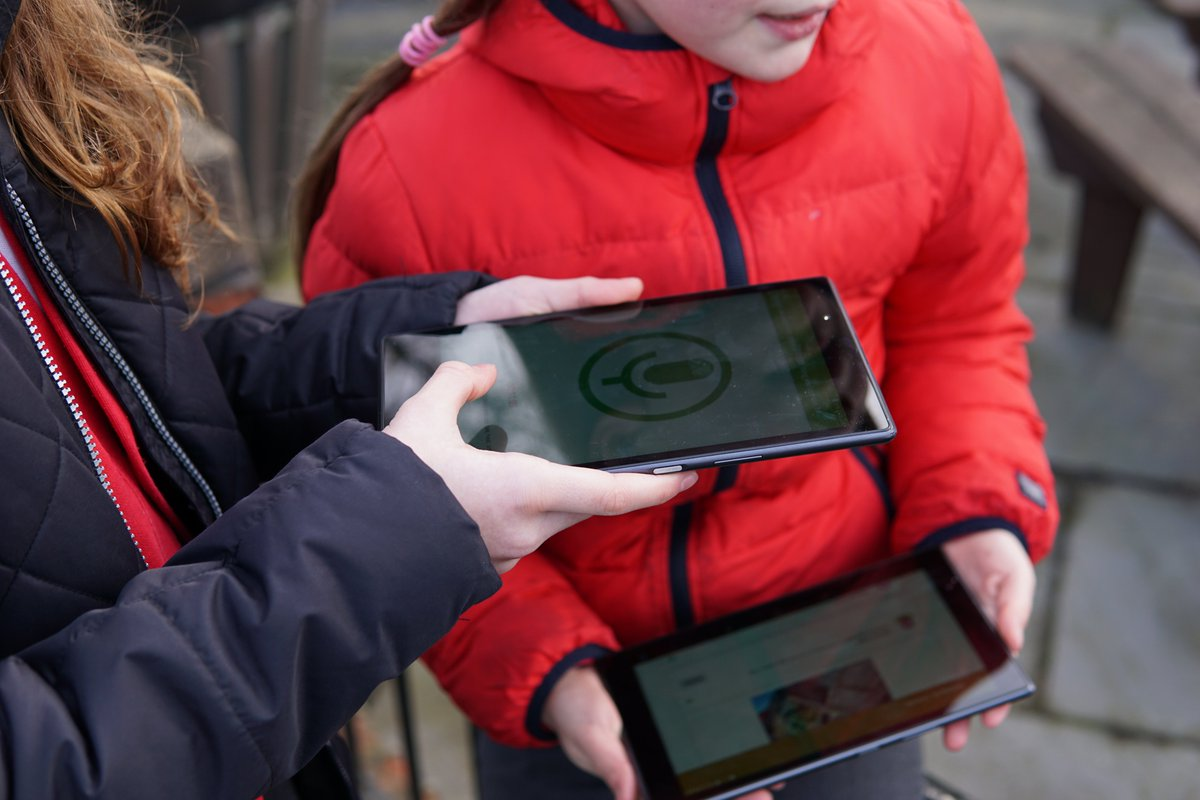
\includegraphics[width=0.8\columnwidth]{images/chapter07/senseExplorers.jpg}
  \caption[Students using OurPlace to log findings during Sense Explorers]{Students using OurPlace to log environmental data readings during the Sense Explorers project.}~\label{fig:SenseExplorers}
\end{figure*}

Several technologies have been used as a part of the design section of the Sense Explorers process. In several implementations, the OurPlace application has been used by students in tandem with a custom Raspberry Pi device. During these activities, students were guided by \textit{Location Hunt} Tasks in a pre-made OurPlace Activity to particular sites of interest, and, through Follow-Up Tasks, asked to take readings from the Raspberry Pi (e.g. air quality, decibel readings). This data could then be logged into the \textit{Text Entry} Follow-Up Tasks, and reflected upon by the students in-situ using the more free-form \textit{Record Audio} and \textit{Record Video} Tasks (Figure \ref{fig:SenseExplorers}). This use of OurPlace demonstrates how it can be used to utilise local space and place as learning resources (\hyperref[DG1]{DG1}), with the children's learning contextualised within their own local environment. After collection, the children's observations and reflections were then uploaded to the OurPlace site, for use in the later stages of Sense Explorers.

As with Teacher 1's `Welcome to Class 2' Activity (Table \ref{tab:TeacherActivities}, row 9), these studies demonstrated that OurPlace can be useful as part of a larger process, and doesn't need to be at the centre of the learner's attention throughout an educational activity to be an effective tool. For example, Teacher 2 used the application to give the students instructions and record their final outcome, while the majority of the students' time was spent discussing the subject and using external tools such as whiteboards. Sense Explorers took this a step further, and made OurPlace a single component within a much larger pipeline---the observations and reflections submitted by students via OurPlace went on to inform their later designs. This pointed towards the potential for creative mobile learning technologies such as OurPlace to be useful as tools within project-based learning (PBL) style pedagogies. Our later explorations of a framework for using place-based mobile learning technologies within all stages of PBL (not just research, but also the creation of a final product) are discussed in Chapter \ref{chap:student-created}.

\subsection{Tyne Fresh Field Trips}
\label{sec:TyneFresh}

\begin{figure*}
  \centering
  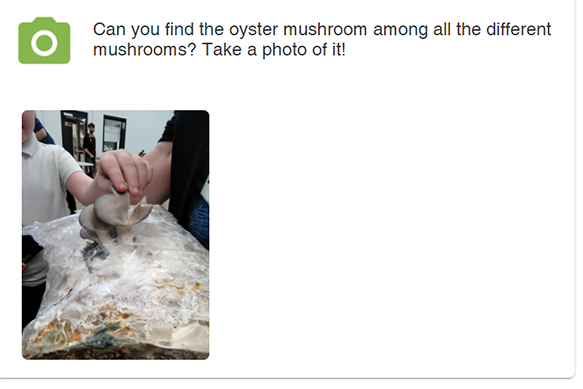
\includegraphics[width=0.8\columnwidth]{images/chapter07/mushroom.png}
  \caption[A student's uploaded photo from a visit to a mushroom producer]{A student's uploaded response to a \textit{Take Photos} task, taken during a school trip to a mushroom producer as a part of the Tyne Fresh project.}~\label{fig:MushroomTrip}
\end{figure*}

As a part of a research project relating to food sustainability and the use participatory design in local food production and consumption \citep{Prost2019}, several researchers at Open Lab have developed the social enterprise `Tyne Fresh'. Developed in partnership with local food producers and a community hub, Tyne Fresh aims to connect the community with local producers---encouraging the consumption of sustainable and healthy produce---and also supports the local food bank with proportional donations.

One of the researchers, Sebastian Prost, has used the OurPlace multiple times during related engagements with school students. The first of these was using the OurPlace app with school students during a field trip to a local mushroom producer. Prior to the trip, Prost worked with the producer to create an OurPlace Activity for the students to complete in pairs on the day. This Activity used Follow-Up Tasks to structure the children visiting different `stations' in the mushroom farm, each concerning a different aspect of food production. Tasks varied from challenging students to find and \textit{Take Photos} of particular types of mushroom (Figure \ref{fig:MushroomTrip}), to \textit{Record Audio} of their reflections and understanding of the sustainable growing processes taught to them on the trip. This Activity was produced by combining the researcher's experience in digital systems with the community member's expert domain knowledge, resulting in an Activity which made good use of the technology through an assortment of interactive Task Types, but also meaningfully engaged with the subject domain. In this way, OurPlace had been used to utilise the knowledge and values of local community members as a learning resource within a formal education context (\hyperref[DG1]{DG1}).

Prost used the OurPlace application during another school trip to the food bank supported by the Tyne Fresh project. This time, rather than the researcher create the Activity with the domain expert, he co-produced it with the students. Prior to the trip, Prost asked the children to prepare questions which they would like to ask the staff at the food bank, or ascertain from their own investigations during the trip. These questions included: `\textit{Does the food bank have to waste or throw out food?}'; `\textit{Are you handing out more food or less every year?}'; and `\textit{How much fresh food compared to tinned food is there at the food bank?}'. A total of 28 of these questions were then inserted into the app as a mix of \textit{Record Audio}, \textit{Multiple Choice} and \textit{Text Entry} Tasks, with each question also crediting the students who submitted it (further supporting the theme of Activity co-production). When asked about his inclusion of the OurPlace app and its role within the class project prior to the trip, Prost said:

\begin{displayquote}
`The kids will work in teams and each team member will have different roles. I’m trying to find a balance between hands-on activities (so they need their hands free), non-digital and digital tools.

In teams of 6-7, three pupils will be “workers”, doing some of the work in a food bank, while the other three document. One of these will be a “journalist” with an iPad to take photos and videos, another will be an “illustrator" with a clipboard, pen \& paper to illustrate the process/how a food bank works. And one will be a “quizmaster” and has the OurPlace app.

Afterwards they’ll use the all the materials to create some paper-based content reflecting on their visit.'
\end{displayquote}

This continued the trend of using OurPlace as a supporting tool within a larger, PBL-style process, with the app being used during the research and resource gathering stages in preparation for the creation of a final product (in this case, the children's paper-based content which reflected upon the role of the food bank, food production and consumption within wider society). However, rather than the OurPlace Activity being produced by the students themselves (as explored in Chapter \ref{chap:student-created}), this was instead co-created with by the children and researcher.

\section{Summary}

This chapter covered the use of ParkLearn and OurPlace within formal education contexts, where teachers and researchers had created Activities for students to complete. These studies aimed to assess the application's success as a design for civic mobile learning, and also investigate new ways in which such technologies could be used. 

Through these studies, the platform was demonstrated to meet its design goals noted in Chapter \ref{chap:Design}: it was shown to be able to utilise place and communities as learning formal education resources through the Sense Explorers and Tyne Fresh projects; the platform was used by teachers seamlessly across multiple contexts, such as the classroom, school grounds and external locations; it shown to be flexible enough to support a variety of pedagogical approaches (with Activity design decisions being able to afford students very little or very large amounts of control over their learning); both adults and children as young as 4 years old were shown to be able to use the application, and it was used by participants such as Teacher 1, who boasted little in the way of technical confidence; the application supported students in situated learning and reflection in authentic contexts, with the added ability to bring those observations and reflections back to the classroom for later use; and its design was iterated upon throughout the studies to provide greater support for device sharing and offline usage by schools with limited resources. 

Teacher 1 noted that the simplified processes and interfaces offered by the application meant that they could once again fit the uploading the children’s work into their workflow, allowing them to promote follow-up classroom activities and even share the children's content in engagements between the school and the surrounding community. Furthermore, through supporting the creativity and independence of students, Teacher 1 argued that the platform promoted their ownership of content, increasing learners’ engagement in follow-up classroom activities. Through a combination of these two factors, Teacher 1 also helped us identify opportunities for mobile learning technologies such as OurPlace to support cross-cultural civic inquiry, encouraging learners to share their values, knowledge and questions in a manner already embraced by citizen science research.

As the platform matured and the studies went on, OurPlace also started being used as a single component within larger processes. For example, Teacher 1 used the application to give the students instructions and record their final outcome, while the majority of the students’ time was spent using external tools such as whiteboards. Sense Explorers took this a step further, with OurPlace existing within larger pipeline. Finally, OurPlace was also used within the Tyne Fresh project as a research and resource gathering tool, in preparation for the subsequent creation of a final product. These uses of the platform all pointed towards the potential for creative mobile learning technologies such as OurPlace to be useful as tools within project-based learning style pedagogies---an application which will be explored in Chapter \ref{chap:student-created}.